\chapter{\term{ROCm} in Dat Centers}

\term{ROCm} 在資料中心和HPC雲端環境中提供無縫支援,使大量節點可以在多個用戶之間共享。\term{ROCm} 為多個平台提供虛擬容器支援,包括Docker、Singularity和Kubernetes。這些平台允許使用者在AMD GPU平台上部署具有 \term{ROCm} 支援的微容器。\term{ROCm} 也提供與雲端環境中的作業排程器的簡易整合,使用諸如簡單Linux資源管理工具(\term{SLURM})和負載共享設施(\term{LSF})等管理框架。在本章中,我們將探討其中一些功能,包括容器和作業排程器在 \term{ROCm} 系統上的應用。

\section{Containerized \term{ROCm}}

\term{ROCm} 虛擬容器為程式設計師提供了一個高效的方式來打包他們的程式碼並與其他程式設計師分享。AMD透過Docker和Singularity為每個新的 \term{ROCm} 版本提供可即時部署的虛擬容器。AMD也提供預裝常用機器學習函式庫如 \term{PyTorch} 和 \term{TensorFlow} 的容器。這使程式設計師可以直接使用這些容器來運行他們的機器學習應用程式,而無需執行耗時的設定。\autoref{fig:12-1} 展示了容器平台如何在 \term{ROCm} 系統上運作。在基礎層面有一個安裝了 \term{ROCm} 及 \term{ROCm} 支援硬體的主機作業系統。接著容器平台運行在主機作業系統之上。最後,各種應用程式(應用程式1、2和3)在平台上通過容器執行。容器處理所有與底層作業系統的資源管理,且應用程式與其他程式互相隔離。有了這個基本認知,我們可以利用具有 \term{ROCm} 支援的Docker容器。首先,我們只需從官方AMD Docker Hub儲存庫下載Docker容器,該儲存庫公開發布不同的ROCm容器。基礎容器以及那些預裝軟體函式庫的容器都有提供。

在我們的例子中,我們使用一個附帶 \term{ROCm} 安裝的Docker容器。重要的是,虛擬容器並不會虛擬化Linux核心。相反地,它提供輕量級且快速的容器化。這對 \term{ROCm} 堆疊(stack)的含義是 \term{ROCm} 核心和相應模組必須安裝在主機上。因為容器共享主機核心,它們也必須在容器外部共享 \term{ROCm} 核心驅動程式功能。在此範例中我們使用來自AMD Docker Hub儲存庫的 \term{rocm-terminal} Docker映像檔。開始時,我們使用\bold{docker pull rocm/rocm-terminal}將映像檔下載到本機系統。然後,我們使用命令\bold{docker run -it --device=/dev/kfd --device=/dev/dri --group-add video rocm/rocm\-terminal}來運行容器,這會在 \term{rocm\-terminal}容器內啟動一個bash shell。最後,我們在 \term{ROCm} 環境中獲得一個工作的Docker容器,程式設計師可以用它來部署他們的應用程式作為微服務。他們也可以使用容器來共享已綁定所有必要依賴項的程式碼。我們鼓勵讀者在Docker Hub上嘗試AMD提供的其他Docker容器。

\begin{figure}[h]
    \centering
    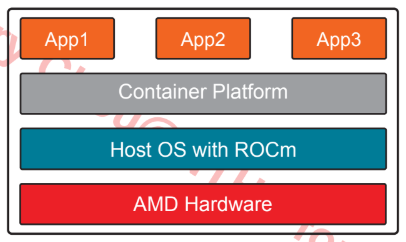
\includegraphics[width=0.75\linewidth]{FileAusiliari//Screenshots/Figure12-1.png}
    \caption{ROCm如何與容器平台整合以實現高效的應用程式部署}
    \label{fig:12-1}
\end{figure}

\section{Managing \term{ROCm} Containers using Kubernetes}

\term{ROCm} 也提供在Kubernetes平台上輕鬆部署虛擬化容器的功能。對於不熟悉Kubernetes的讀者來說,它基本上是一個容器編排服務。例如,如果一個組織已經部署了大量的容器作為微服務,手動管理這些容器將會非常繁瑣,他們可以將這些容器部署到Kubernetes上,這樣可以減輕管理和編排的負擔。Kubernetes還提供故障容錯和可擴展性功能。

\begin{figure}[h]
    \centering
    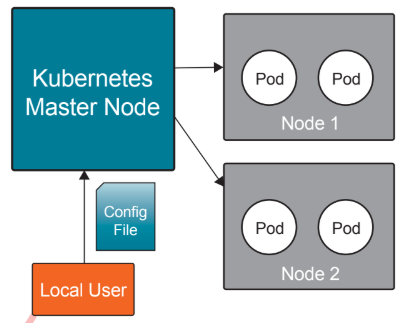
\includegraphics[width=0.75\linewidth]{FileAusiliari//Screenshots/Figure12-2.png}
    \caption{使用Kubernetes的系統之高階架構。使用者透過配置文件與主節點進行通訊。主節點負責管理和調度跨節點的Pods。}
    \label{fig:12-2}
\end{figure}

在Kubernetes上運行的一組容器被稱為「Pod」。系統管理員或程式設計師需描述管理Pod所需的所有內容,包括建立新容器、終止現有容器,以及擴展和升級Pod。\autoref{fig:12-2} 顯示了Kubernetes系統的高階架構。本地使用者透過描述所需容器、資源限制等的配置文件與主節點通訊。Kubernetes主節點(可以有多個)管理並在系統中的不同節點間調度它們。在微服務架構的系統中,Kubernetes根據日曆需求來調整資源。使用Kubernetes有許多優點,但詳細描述超出了本書的範圍。

為了利用Kubernetes容器編排,\term{ROCm} 為AMD GPUs提供支援,使程式設計師能夠在 \term{ROCm} 支援的GPUs上利用此技術。AMD在Docker hub儲存庫上提供了一個Kubernetes設備插件,支援透過容器集群進行GPU註冊以用於計算目的。從Docker pull此插件後,程式設計師必須確保它在具有 \term{ROCm} 支援GPU的所有節點上執行。為了簡化這個過程,應該使用 \term{Daemonset} 工具,因為它能讓Pod副本在集群中的所有節點上運行。AMD的Github儲存庫中的Kubernetes設備插件提供了一個名為\bold{k8s-ds-amdgpu-dp.yaml}的yaml檔案用於此目的。程式設計師運行\bold{kubectl create -f k8s-ds-amdgpu-dp.yaml}來拉取它。讀者可以在 \cite{Kubernetes-Documentation} 了解更多關於Daemonset的工作原理。

在 \term{Daemonset} 運行之後,我們部署一個在GPU上運行AlexNet基準測試的pod。部署後,pod會進入睡眠狀態。AlexNet是一個用於圖像分類的DNN。用於創建此Pod的yaml檔案如 \lstref{lst:config_file+exe_alexnetink8s} 所示。從第8行開始,我們可以看到負責指定容器名稱(第9行)和容器的Docker映像檔(第10行)的部分。第14行標識將運行容器的GPU,在這個案例中設為零。接著是實際的AlexNet基準測試腳本,它將在容器內運行。最後,第17-19行指定了pod的資源限制,即單個GPU。要運行yaml檔案,程式設計師首先需要啟動並運行該pod。這可以通過命令\bold{kubectl create -f alexnet-tf-gpu.yaml}來完成。使用\bold{kubectl describe pods}可以檢查pod的狀態。最後,要查看AlexNet訓練腳本的結果,我們運行\bold{kubectl logs alexnet-tf-gpu-pod alexnet-tf-gpu-container},其中「\bold{alexnet-tf-gpu-pod}」指的是Pod名稱,「\bold{alexnet-tf-gpu-container}」指的是yaml檔案中指定的容器名稱。

這個例子展示了在 \term{ROCm} 支援的GPU上使用Kubernetes框架部署容器是多麼容易。我們鼓勵讀者通過更改yaml檔案的參數並嘗試自己預構建的容器來進行實驗。

\begin{lstlisting}[language=yaml, caption={在Kubernetes平台上執行AlexNet基準測試的配置文件}, captionpos=t, label={lst:config_file+exe_alexnetink8s}]
apiVersion: v1
kind: Pod
metadata:
    name: alexnet-tf-gpu-pod
    labels:
        purpose: demo-tf-amdgpu
spec:
    containers:

        - name: alexnet-tf-gpu-container
          image: rocm/tensorflow:latest
          workingDir: /root
          env:
          - name: HIP_VISIBLE_DEVICES
            value: "0" # # 0,1,2,...,n for running on GPU and select the GPUs, -1 for running on CPU
          command: ["/bin/bash", "-c", "--"]
          args: ["python3 benchmarks/scripts/tf_cnn_benchmarks/tf_cnn_benchmarks.py --model=alexnet; trap : TERM INT; sleep infinity & wait"]
          resources:
            limits:
              amd.com/gpu: 1 # requesting a GPU
\end{lstlisting}

\begin{figure}[h]
    \centering
    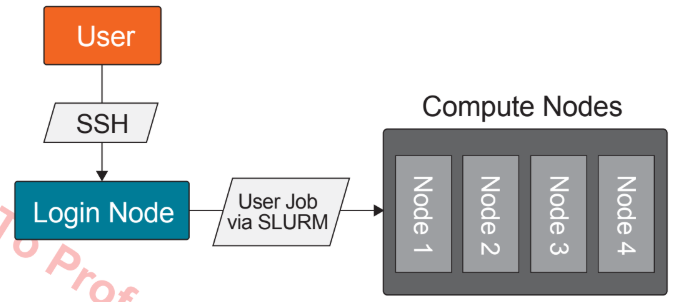
\includegraphics[width=0.75\linewidth]{FileAusiliari//Screenshots/Figure12-3.png}
    \caption{基於 \term{SLURM} 的集群運作方式的高階概述。程式設計師登入節點並透過 \term{SLURM} 提交作業,這些作業隨後由 \term{SLURM} 在計算節點上進行調度和執行。}
    \label{fig:12-3}
\end{figure}

\section{Managing \term{ROCm} Nodes using \term{Slurm}}

具有 \term{ROCm} 功能的GPU也可以使用調度工具來管理,例如 \term{SLURM}。這類工具在HPC中心和學術計算集群中被廣泛用於管理共享資源的存取。在本節中,我們將探討一些基本的 \term{SLURM} 功能,包括如何請求互動式存取 \term{ROCm} GPU以及如何向其提交job。

兩個重要的集群相關術語需要理解的是「主節點」和「計算節點」。當使用者登入集群時,其主節點是第一個位置,也就是登入節點。從那裡,使用者可以向 \term{SLURM} 發出請求以存取計算節點,以便運行他們的作業。\autoref{fig:12-3} 顯示了運行 \term{SLURM} 的集群的高階區塊圖。

使用者可以透過兩種方式向 \term{SLURM} 發出請求。第一種是透過 \term{SLURM} 互動模式,它允許使用者在請求的節點上開啟遠端終端機。從那裡,使用者可以執行任務,例如編譯程式碼、安裝函式庫和執行程式。第二種是透過批次提交模式,在這種模式下,程式設計師建立一個包含計算和記憶體資源請求、當資源可用時要執行的命令,以及作業時間限制的批次腳本。使用批次模式時,作業會提交給 \term{SLURM} 排程器,由它進行排隊和管理。使用者也可以在批次腳本中包含在作業完成時通知他們的命令。接下來我們將查看這些模式的範例。 

\subsection{\term{SLURM} interactive mode}

要在互動模式中執行,請求資源的命令是 \bold{salloc}。它有幾個可選參數,可以在官方 \term{SLURM} 文件中查看,或者只需運行 \bold{salloc -h} 即可列出選項。就我們的目的而言,三個最重要的參數包括 \bold{-N},即節點數量,\bold{-p},即請求的分區,以及 \bold{-t},即作業的時間限制。例如,命令 \bold{salloc -N 2 -p M1100 -t 02:00:00} 表示我們正在請求M1100分區上的兩個節點,時間為2小時。這個命令是阻塞型的,意味著它只會在請求被 \term{SLURM} 處理後才返回。然後,使用者透過終端機直接登入到請求的計算節點。當時間限制到期時,終端機會自動退出並顯示超時訊息,使用者返回他們的主節點。如果使用者在超時之前完成,他們可以發出 \bold{scancel <JOB\_ID>},其中「job ID」指的是使用者的作業。可以通過 \bold{squeue -u \$USER} 找到作業ID。

\subsection{\term{SLURM} batch submission mode}

在 \term{SLURM} 的批次提交模式中,程式設計師準備一個類似於 \term{matmul.bash} 的腳本,如 \lstref{lst:slurm_job_example} 所示。在此,我們指定集群分區、GPU數量、記憶體量和執行時間。除了這些細節之外,我們需要指定腳本應該載入 \term{ROCm} 模組,以便正確設定環境來使用所有與 \term{ROCm} 相關的函式庫。我們在第18行包含編譯命令。在此範例中,我們編譯 \term{matmul.cpp},它會產生 \term{matmul} 二進位檔。最後,在第20行,我們指定應該執行 \term{matmul} 的腳本。要請求 \term{SLURM} 調度和執行我們的作業,我們只需使用 \bold{sbatch} 命令並傳入檔案名稱。在這個案例中,\bold{sbatch matmul.bash} 將作業提交給 \term{SLURM} 調度器。如果程式輸出到 \term{stdout},結果會儲存在 \term{gpu.out} 檔案中(\term{matmul.bash} 的第4行)。

\begin{lstlisting}[language=bash, caption={matmul.bash \term{SLURM} 批次提交腳本。}, captionpos=t, label={lst:slurm_job_example}]
#!/bin/bash

#SBATCH --job-name=matmulgpu   # job name
#SBATCH --output=gpu.out       # output log file
#SBATCH --error=gpu.err        # error file  
#SBATCH --time=01:00:00        # 1 hour of wall time
#SBATCH --nodes=1              # 1 GPU node
#SBATCH --partition=m1100      # GPU2 partition
#SBATCH --ntasks=1             # 1 CPU core to drive GPU
#SBATCH --gres=gpu:1           # Request 1 GPU
#SBATCH --mem=8Gb.            # Request 8 GB of memory

# Load all required modules below. As an example, we load rocm:
module load rocm

# Add lines here to run your GPU-based computations.
hipcc matmul.cpp -o matmul

./matmul
\end{lstlisting}

\section{Conclusion}

在本章中,我們學習了如何在資料中心環境中使用 \term{ROCm}。無論我們使用Docker、Kubernetes,還是 \term{SLURM} 調度器,\term{ROCm} 都為資料中心提供了所有必要的服務支援,使微服務能夠快速部署和擴展。此外,它也為系統管理員簡化了集群和資料中心的管理。